%% ------------------------------------------------------------
%% TITLE:     Vibrations and Waves - Summary of Three Types of Signal Oscillations
%% AUTHOR:    BINGHUAN W LI (Dept. Chemical Eng/Bio Eng, Imperial)
%% COMPILED:  XeLaTeX with TeX Live version 2023
%% LICENSE:   This work is licensed under a Creative Commons Attribution-NonCommercial 4.0 International License.
%% ------------------------------------------------------------

% Version History:
% v1.0  - xxxx-xx-xx - Initial draft
% v1.1  - 2024-11-06 - Reformatted the document

\documentclass[12pt,a4paper]{article}
\usepackage[margin=2cm]{geometry}
\usepackage{fontspec}
    \setmainfont{Times New Roman}
\usepackage{newtxmath}
\usepackage{amsmath, amsfonts, cancel}
\usepackage{enumitem}
\usepackage{float}

\usepackage{xcolor}
    \definecolor{linkcolour}{rgb}{0,0.2,0.6}
\usepackage[breakable]{tcolorbox}
% \usepackage{booktabs}
\usepackage{hyperref}
    \hypersetup{colorlinks,
                breaklinks,
                urlcolor=linkcolour,
                linkcolor=black,
                citecolor=black,
                pdftitle={Vibrations and Waves},
                pdfauthor={Li, Binghuan}}

            
\usepackage{tikz}
\usetikzlibrary{calc,patterns,decorations.pathmorphing,decorations.markings}
\usepackage[siunitx]{circuitikz}
\usetikzlibrary{arrows}

\usepackage{titling}
\setlength{\droptitle}{-4em}
\graphicspath{{./images/}}
\setlength\parindent{0pt}
\linespread{1.15}

%=====================================================%
\begin{document}
\title{\textbf{Vibrations and Waves} \\ Summary of Three Types of Signal Oscillations}
\author{Binghuan Li\\ \href{mailto:binghuan.li19@imperial.ac.uk}{\texttt{binghuan.li19@imperial.ac.uk}}}
\date{\today}
\maketitle
%=================Undamped Oscillation=================%
\section{Free/Undamped Oscillation}

\begin{figure}[H]
    \centering
    \begin{tikzpicture}[every node/.style={draw,outer sep=0pt,thick}]
        \tikzstyle{spring}=[thick,decorate,decoration={zigzag,pre length=0.3cm,post length=0.3cm,segment length=6}]
        \tikzstyle{ground}=[fill,pattern=north east lines,draw=none,minimum width=0.75cm,minimum height=0.3cm]
        \node (M) [minimum width=1.5cm, minimum height=1.5cm] {$m$};
        \node (wall) [ground, rotate=-90, minimum width=1.5cm,yshift=-3cm] {};
        \draw (wall.north east) -- (wall.north west);
        \node (gnd) [ground, rotate=0, minimum width=5cm,yshift=-0.9cm, xshift=-0.65cm] {};
        \draw (wall.south east) -- (M.south east)--+(1.1cm,0);
        \draw [spring] (wall.100) -- ($(M.north west)!(wall.100)!(M.south west)$);
        \node[above, draw=none] at (-2.1,0.2){$k$};
    \end{tikzpicture}

    \caption{A spring-mass mechanical system}
    \label{fig:spring-mass}
\end{figure}

The equilibrium state of the system shown in \autoref{fig:spring-mass} can be mathematically described by Hooke's law:
\begin{equation} \label{eqn:1}
    F = ma = -kx
\end{equation}
Re-arrange \autoref{eqn:1}, we could get
\begin{equation} \label{eqn:2}
    ma + kx = 0
\end{equation}

The acceleration, $a$, is the second-derivative of the displacement, $x$, with respect to the time, $t$: $\displaystyle a=\frac{d^{2}x}{dt^{2}}$. So \autoref{eqn:2}  can be converted to a \textit{2\textsuperscript{nd}-order ordinary differential equation}:
\begin{equation} \label{eqn:3}
    m\frac{d^{2}x}{dt^{2}}+kx=0
\end{equation}
\autoref{eqn:3} is commonly referred to as the \textit{governing equation} that describes the dynamic behaviours of the mechanical system shown in \autoref{fig:spring-mass}. This equation is now ready to be solved!

%% solution procedure
\begin{tcolorbox}[breakable, title=Solution Procedure]
The coefficient of the 2\textsuperscript{nd}-order derivative term becomes 1 if we divide the mass $m$ in \autoref{eqn:3}, 
\begin{equation} \label{eqn:4}
    \frac{d^{2}x}{dt^{2}}+\frac{k}{m}x=0  
\end{equation}

Applying the \textit{trial solution} $\displaystyle x = A\cos (\omega t+ \phi)$ to \autoref{eqn:4}\footnote{Well... for now you just need to accept that this solution is correct!}:
\begin{equation} \label{eqn:5}
    \underbrace{-A\omega^{2}\cos(\omega t+ \phi)}_{\ddot{x} = {d^{2}x}/{dt^{2}}} + \frac{k}{m} \underbrace{A\cos(\omega t+\phi)}_{x}=0
\end{equation}

Re-arrange \label{eqn:5}, we could separate a common, non-zero term $\cos(\omega t+\phi)$: 
\begin{equation} \label{eqn:6}
(-\omega^{2}+ \frac{k}{m}) \underbrace{A \cdot \cos(\omega t+\phi)}_{\text{this term cannot be zero!}} = 0
\end{equation}

\autoref{eqn:6} implies that only the first term $\displaystyle (-\omega^{2}+ \frac{k}{m})$ is zero (since the cosine term can \textit{never} be zero!). Therefore, we can express $\omega$ in terms of $k$ and $m$:
\begin{equation} \label{eqn:7}
-\omega^{2}+ \frac{k}{m}=0 \quad \to \quad 
\boxed{\omega = \pm \sqrt{\frac{k}{m}}}
\end{equation}

\textit{We are only interested in the positive solution of $\omega$!} Therefore, the solution for \autoref{eqn:3} is
\begin{equation} \label{eqn:8}
    \boxed{x = A\cos (\sqrt{\frac{k}{m}}t+\phi)}
\end{equation}
\end{tcolorbox}

\autoref{eqn:8} is the general solution for a \textbf{undamped system}. Let us visualise this by plotting the displacement as a function of time ($x$-$t$):
\begin{figure}[H]
    \centering
    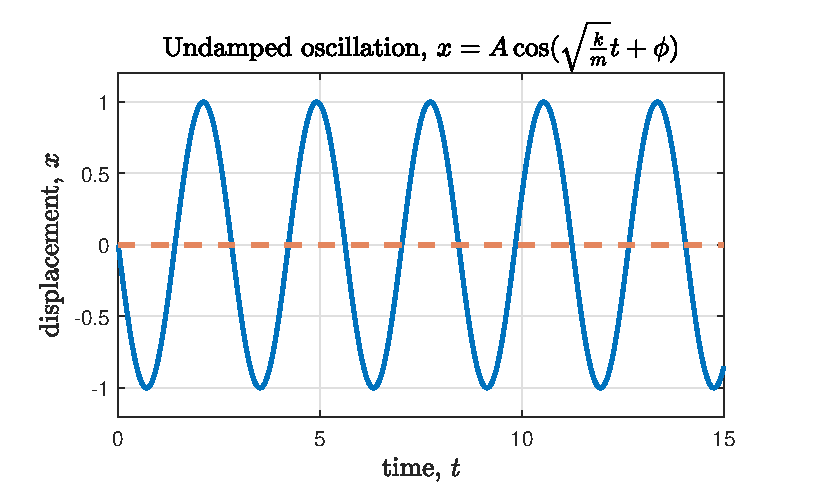
\includegraphics[width=.7\textwidth]{undamped_oscillation.eps}
    \label{fig:my_label}
\end{figure}
As you can see, there is no decay of the displacement as time goes by, \textit{i.e.}, the amplitude of the displacement is constant due to the absence of the damping effects. The mass in the spring-mass system will move back and forth with perfect conservation of energy! \\

\hrule \vspace{.1cm}
\paragraph{Electrical analogy} The electrical equivalent circuit that can generate the free oscillation is a capacitance ($C$) -inductance ($L$) circuit. 
\begin{figure}[H]
    \centering
    \begin{tikzpicture}
    \draw
    	(0,2) 
    	to[C=$C$] ++(3,0)
    	to[L = $L$] ++(0,-2)
    	--(0,0);
     \draw[>=angle 90,<->,red, shorten <=1mm, shorten >=1mm] (0,0) to node [fill=white] {$V_{total}$} (0,2);
    \end{tikzpicture}
\end{figure}
The voltage across 
\begin{itemize}
    \item the inductor, $L$: $\displaystyle V_{L} = L\frac{dI}{dt}$
    \item the capacitor, $C$: $\displaystyle V_{C} = \frac{1}{C}\int_{0}^{t} I(\tau) d\tau$
\end{itemize}
By Kirchhoff's voltage law:
\[
    V_L + V_C = V_{total} \quad \to \quad L \frac{dI}{dt} + \frac{1}{C}\int_{0}^{t} I(\tau) d\tau = V_{total} 
\]
Differentiate:
\[
    L \frac{d^2I}{dt^2} + \frac{1}{C}I = 0
\]
which is the governing equation for the above $L$-$C$ system.\\

% To compare the equivalent components:
% \begin{table}[H]
%     \centering
%     \begin{tabular}{c c}
%     \toprule
%     mechanical system component  &   electrical system component \\
%     \midrule
%         mass, $m$ &  inductor, $L$  \\
%         spring, $k$ & capacitor, $C$    \\
%         displacement, $x$  &   electrical charge, $q$ \\
%         time, $t$   &   time, $t$ \\
%     \bottomrule
%     \end{tabular}
% \end{table}
%=================Damped Oscillation=================%
\newpage
\section{Damped Oscillation}

\begin{figure}[H]
    \centering
    \begin{tikzpicture}[every node/.style={draw,outer sep=0pt,thick}]
    \tikzstyle{spring}=[thick,decorate,decoration={zigzag,pre length=0.3cm,post length=0.3cm,segment length=6}]
    \tikzstyle{damper}=[thick,decoration={markings,  
      mark connection node=dmp,
      mark=at position 0.5 with 
      {
        \node (dmp) [thick,inner sep=0pt,transform shape,rotate=-90,minimum width=15pt,minimum height=3pt,draw=none] {};
        \draw [thick] ($(dmp.north east)+(2pt,0)$) -- (dmp.south east) -- (dmp.south west) -- ($(dmp.north west)+(2pt,0)$);
        \draw [thick] ($(dmp.north)+(0,-5pt)$) -- ($(dmp.north)+(0,5pt)$) ; 
      }
    }, decorate]
    \tikzstyle{ground}=[fill,pattern=north east lines,draw=none,minimum width=0.75cm,minimum height=0.3cm]
    \node (M) [minimum width=1.5cm, minimum height=1.5cm] {$m$};
    \node (wall) [ground, rotate=-90, minimum width=1.5cm,yshift=-3cm] {};
    \draw (wall.north east) -- (wall.north west);
    \node (gnd) [ground, rotate=0, minimum width=5cm,yshift=-0.9cm, xshift=-0.65cm] {};
    \draw (wall.south east) -- (M.south east)--+(1.1cm,0);
    \draw [spring] (wall.160) -- ($(M.north west)!(wall.160)!(M.south west)$);
    \draw [damper] (wall.20) -- ($(M.north west)!(wall.20)!(M.south west)$);
    \node[below, draw=none] at (-2.1,-0.1){$c$};
    \node[above, draw=none] at (-2.1,0.5){$k$};
    \end{tikzpicture}

    \caption{A spring-mass-damper mechanical system}
    \label{fig:spring-mass-damper}
\end{figure}

\autoref{fig:spring-mass-damper} shows a spring-mass-damper ($k$-$m$-$c$) system. The equilibrium state of the system can be mathematically described by:
\begin{equation} \label{eqn:9}
    F = ma = -cv -kx 
\end{equation}
where $c$ is known as the \textit{damping coefficient}, $v$ is the moving speed of the mass, and $c \cdot v$ is defined as the force exerted by the mechanical damper. Re-arrange \autoref{eqn:9}, we could get
\begin{equation} \label{eqn:10}
    ma + cv + kx = 0
\end{equation}

The velocity, $v$ and the acceleration, $a$ are defined as the 1\textsuperscript{st} and 2\textsuperscript{nd} derivative of the displacement, $x$, with respect to the time, $t$:  $\displaystyle v=\frac{dx}{dt}$, $\displaystyle a=\frac{d^{2}x}{dt^{2}}$. Therefore, \autoref{eqn:10} can be converted to a \textit{2\textsuperscript{nd}-order ordinary differential equation} (again!)
\begin{equation} \label{eqn:11}
    m\frac{d^{2}x}{dt^{2}} + c\frac{dx}{dt} + kx = 0
\end{equation}

%% solution procedure
\begin{tcolorbox}[breakable, title=Solution Procedure]
The coefficient of the 2\textsuperscript{nd}-order derivative term becomes 1 if we divide the mass $m$ in \autoref{eqn:11}, 
\begin{equation} \label{eqn:12}
    \frac{d^{2}x}{dt^{2}} + \frac{c}{m} \frac{dx}{dt} + \frac{k}{m}x = 0
\end{equation}

Let us first define two parameters: \textit{natural frequency} and \textit{damping factor}:
\begin{itemize}
    \item Natural frequency, $\displaystyle \omega_{n} = \sqrt{\frac{k}{m}}$
    \item Damping factor, $\displaystyle \gamma = \frac{c}{2\sqrt{km}}$
\end{itemize}

If we apply the natural frequency and damping factor defined above to \autoref{eqn:12}, we will obtain a more \textit{generic} expression of the governing equation: 
\begin{equation} \label{eqn:13}
    \frac{d^{2}x}{dt^{2}} + 2\gamma \omega_{n}\frac{dx}{dt} + \omega_{n}^{2}x=0
\end{equation}

To solve \autoref{eqn:13}, we shall apply the trial solution $\displaystyle x = Ae^{\mu t}$ to \autoref{eqn:13}\footnote{Let us assume this trial solution is correct for now!}.
\begin{equation} \label{eqn:14}
    \underbrace{\mu^{2}Ae^{\mu t}}_{\ddot{x}} \ + \ 2\gamma\omega_{n} \underbrace{\mu Ae^{\mu t}}_{\dot{x}} \ + \ \omega_{n}^{2} \underbrace{Ae^{\mu t}}_{x} = 0
\end{equation}

Re-arrange \label{eqn:14}, we could separate a common, non-zero term $Ae^{\mu t}$: 
\begin{equation} \label{eqn:15}
    (\mu^{2}+2\gamma\omega_{n}\mu+\omega_{n}^{2}) \underbrace{A\cdot e^{\mu t}}_{\text{non-zero!}} = 0
\end{equation}

\autoref{eqn:15} implies that only the first term $\displaystyle (\mu^{2}+2\gamma\omega_{n}\mu+\omega_{n}^{2})$ is zero (since the exponential term can \textit{never} be zero!). Therefore, we can solve the quadratic equation of $\mu$ to solve $\mu$ in terms of $\gamma$ and $\omega_n$:
\begin{equation} \label{eqn:16}
    \mu^{2}+2\gamma\omega_{n}\mu+\omega_{n}^{2} = 0
    \quad \to \quad 
    \boxed{\mu = -\gamma \omega_{n}\pm \omega_{n}\sqrt{\gamma^{2}-1}}
\end{equation}

What is the general solution to displacement? \textbf{we need to consider three conditions of $\gamma^{2}-1$} (the term under the square root), \textbf{as they correspond to 3 different types of damping effects.}
\end{tcolorbox}

\subsection{Condition 1: $\gamma^{2}-1<0$ - Light Damping}
If $\gamma^{2}-1<0$, the general solution of a 2\textsuperscript{nd}-order ODE should hold the format 
\[
    x = e^{\mu t} (A_1 \cos(\omega_n x) + iA_2\sin(\omega_n x))
\]
\textit{i.e.}, the solution \textit{might be} a complex number.\\

To determine this, for convenience, we first define $\omega_{d}=\omega_{n}\sqrt{1-\gamma^{2}}$,
\begin{align}
\begin{split} \label{eqn:17}
x &= A_{1}e^{\mu_{1}t} + A_{2}e^{\mu_{2}t} \\
& = A_{1}e^{(-\gamma \omega_{n}+j\omega_{d})t}  +A_{2}e^{(-\gamma \omega_{n}-j\omega_{d})t}\\
&= e^{-\gamma \omega_{n} t}\bigg(A_{1}\big(\cos(\omega_{d}t)+j\sin(\omega_{d}t)\big)+A_{2}\big(\cos(\omega_{d}t)-j\sin(\omega_{d}t)\big)\bigg)\\
&= e^{-\gamma \omega_{n} t}\bigg[ \underbrace{(A_{1}+A_{2})}_{C= N\cos\phi}\cos(\omega_{d}t) + \underbrace{j(A_{1}-A_{2})}_{-D=-N\sin \phi}\sin(\omega_{d}t)\bigg]\\
&= e^{-\gamma \omega_{n} t} \big( N\cos\phi \cos\omega_{d}t - N\sin\phi \sin\omega_{d}t \big)\\
& = \boxed{e^{-\gamma \omega_{n} t} N \cos(\omega_{d}t+\phi)}
\end{split}
\end{align}
To plot $x$ against $t$:
\begin{figure}[H]
    \centering
    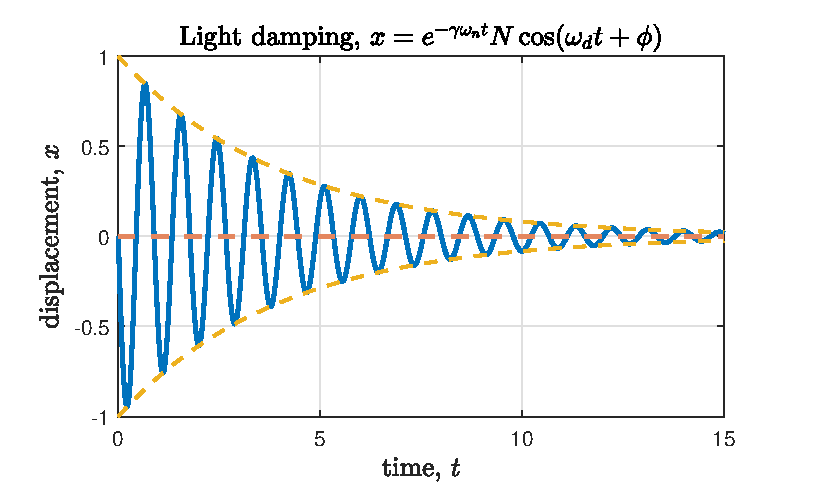
\includegraphics[width=.7\textwidth]{light_damping.eps}
    \label{fig:light_damping}
\end{figure}

Two observations we can make here:
\begin{enumerate}
    \item the occurrence of oscillations, this is described by the cosine term in \autoref{eqn:17}; and

    \item the amplitude of oscillation decays with time (damped) - this is due to the exponential term in \autoref{eqn:17}. The yellow envelops shown in \autoref{fig:light_damping} are exactly the plot of $e^{-\omega_{n}\gamma t}$ and $-e^{-\omega_{n}\gamma t}$.
\end{enumerate}
This type of damping oscillation is commonly known as the \textbf{light damping}.

\subsection{Condition 2: $\gamma^{2}-1>0$ - Heavy Damping}
If $\gamma^{2}-1>0$, there are two distinct roots of $\mu$, therefore, the general solution becomes
\begin{equation}
    \boxed{x = A_{1} e^{\mu_{+} t} + A_{2} e^{\mu_{-} t} = 
    A_{1}e^{-(\gamma \omega_{n}+\omega_{n}\sqrt{\gamma^{2}-1})t}+ A_{2}e^{-(\gamma \omega_{n}-\omega_{n}\sqrt{\gamma^{2}-1})t}}
\end{equation}
To plot $x$ against $t$:
\begin{figure}[H]
    \centering
    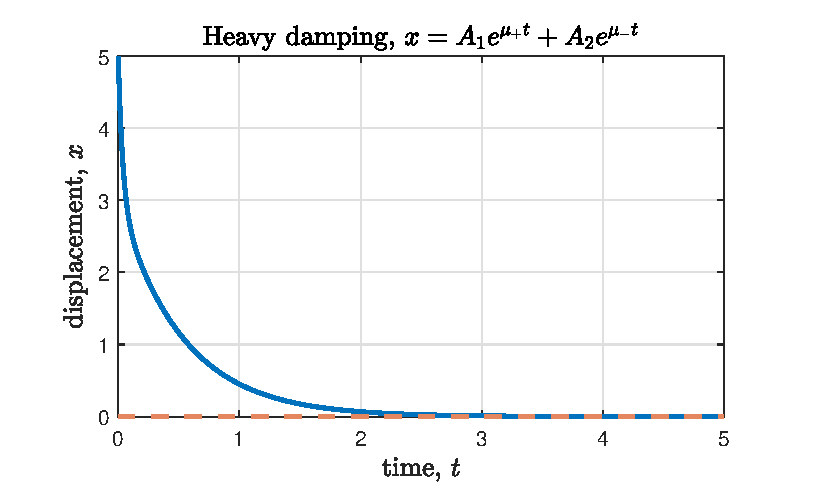
\includegraphics[width=.7\textwidth]{heavy_damping.eps}
    \label{fig:heavy_damping}
\end{figure}

The mass attains its equilibrium gradually \textbf{without} any oscillation. This is known as the \textbf{heavy damping}.

\subsection{Condition 3: $\gamma^{2}-1=0$ - Critical Damping}
If $\gamma^{2}-1 = 0$, the general solution of a 2\textsuperscript{nd}-order ODE should hold the format 
\begin{equation}
    \boxed{x =  (A_1 + A_2 t) e^{\mu t}}
\end{equation}
where in this situation, $\mu = -\omega_{n}\gamma$. To plot $x$ against $t$:
\begin{figure}[H]
    \centering
    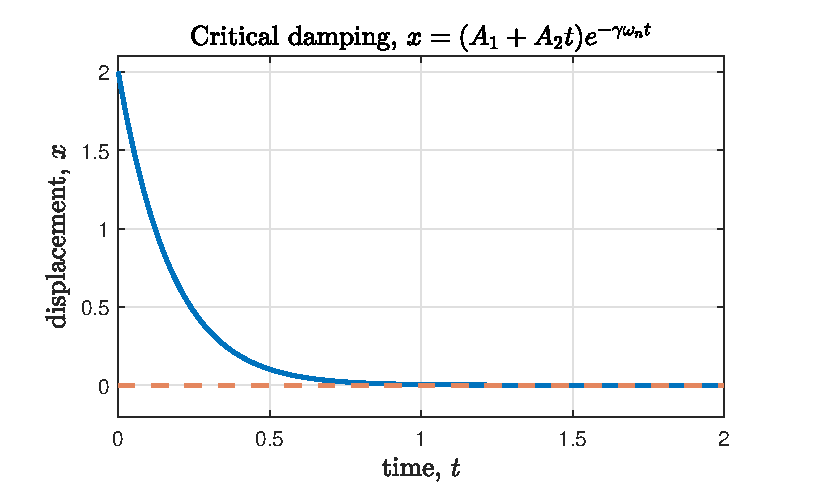
\includegraphics[width=.7\textwidth]{crit_damping.eps}
    \label{fig:crit_damping}
\end{figure}

The mass returns to the equilibrium position as quickly as possible (\textit{i.e.}, quickly within 1 oscillation). This is known as the \textbf{critical damping}. It is the threshold between heavy damping and light damping.\\

\hrule \vspace{.1cm}
\paragraph{Electrical analogy} Three types of damped oscillations can be generated with the following $L$-$C$-$R$ circuit:
\begin{figure}[H]
    \centering
    \begin{tikzpicture}
    \draw
    ++(0,2)
        to[R=\(R\)] ++(2,0) 
        to[L=\(L\)] ++(2,0) 
        to[C=\(C\)] ++(0,-2) 
      -- (0,0);
    \draw[>=angle 90,<->,red, shorten <=1mm, shorten >=1mm] (0,0) to node [fill=white] {$V_{total}$} (0,2);
    \end{tikzpicture}
\end{figure}

The voltage across 
\begin{itemize}
    \item the resistor, $R$: $\displaystyle V_{r} = RI$
    \item the inductor, $L$: $\displaystyle V_{L} = L\frac{dI}{dt}$
    \item the capacitor, $C$: $\displaystyle V_{C} = \frac{1}{C}\int_{0}^{t} I(\tau) d\tau$
\end{itemize}
By Kirchhoff's voltage law:
\[
    V_R + V_L + V_C = V_{total} \quad \to \quad RI + L \frac{dI}{dt} + \frac{1}{C}\int_{0}^{t} I(\tau) d\tau = V_{total} 
\]
Differentiate:
\[
    L \frac{d^2I}{dt^2} + R\frac{dI}{dt} + \frac{1}{C}I = 0
\]
which is a second-order, homogeneous differential equation. To solve this ODE, the corresponding auxiliary equation is
\[
    Lm^2 + Rm + \frac{1}{C} = 0
\]
which yields two solutions
\[
    m_{1, 2} = \frac{-R}{2L} \pm \frac{\sqrt{R^2 - 4L/C}}{2L}
\]
we need to discuss the value of $\sqrt{R^2 - 4L/C}$ to determine the type of damping:
\begin{itemize}
    \item $R^2 > 4L/C$: heavy damping
    \item $R^2 < 4L/C$: under damping
    \item $R^2 = 4L/C$: critical damping
\end{itemize}

%=================Forced Oscillation=================%
\newpage
\section{Forced Oscillation}
So far, we have considered both undamped oscillation and damped oscillation - no further external force was applied once the system was released from the initial position. How will system dynamic behaves if we apply an external force to the system periodically?
\begin{figure}[H]
    \centering
    \begin{tikzpicture}[every node/.style={draw,outer sep=0pt,thick}]
    \tikzstyle{spring}=[thick,decorate,decoration={zigzag,pre length=0.3cm,post length=0.3cm,segment length=6}]
    \tikzstyle{damper}=[thick,decoration={markings,  
      mark connection node=dmp,
      mark=at position 0.5 with 
      {
        \node (dmp) [thick,inner sep=0pt,transform shape,rotate=-90,minimum width=15pt,minimum height=3pt,draw=none] {};
        \draw [thick] ($(dmp.north east)+(2pt,0)$) -- (dmp.south east) -- (dmp.south west) -- ($(dmp.north west)+(2pt,0)$);
        \draw [thick] ($(dmp.north)+(0,-5pt)$) -- ($(dmp.north)+(0,5pt)$) ; 
      }
    }, decorate]
    \tikzstyle{ground}=[fill,pattern=north east lines,draw=none,minimum width=0.75cm,minimum height=0.3cm]
    
    \node (M) [minimum width=1.5cm, minimum height=1.5cm] {$m$};
    
    \node (wall) [ground, rotate=-90, minimum width=1.5cm,yshift=-3cm] {};
    \draw (wall.north east) -- (wall.north west);
    
    \node (gnd) [ground, rotate=0, minimum width=5cm,yshift=-0.9cm, xshift=-0.65cm] {};
    \draw (wall.south east) -- (M.south east)--+(1.1cm,0);
    
    \draw [spring] (wall.160) -- ($(M.north west)!(wall.160)!(M.south west)$);
    \draw [damper] (wall.20) -- ($(M.north west)!(wall.20)!(M.south west)$);
    
    \draw [-latex,ultra thick] (M.east) ++ (0.2cm,0) -- +(1.1cm,0) node [above, draw=none]{$F_{0} \cos \omega t$} ;
    \node[below, draw=none] at (-2.1,-0.1){$c$};
    \node[above, draw=none] at (-2.1,0.5){$k$};
    \end{tikzpicture}

    \caption{A spring-mass-damper mechanical system subjected to a periodic force}
    \label{fig:spring-mass-damper-force}
\end{figure}

\autoref{fig:spring-mass-damper-force} shows a spring-mass-damper ($k$-$m$-$c$) system subjected to a periodic external force $F(t) = F_0 \cos \omega t$. The equilibrium state of the system can be mathematically described by:
\begin{equation} \label{eqn:20}
    F_{total} = ma = -cv - kx + F_{0}\cos\omega t
\end{equation}

Re-arrange \autoref{eqn:20}, we could get
\begin{equation} \label{eqn:21}
    ma + cv + kx = F_{0}\cos\omega t
\end{equation}

Similarly, the velocity, $v$ and the acceleration, $a$ are defined as the 1\textsuperscript{st} and 2\textsuperscript{nd} derivative of the displacement, $x$, with respect to the time, $t$:  $\displaystyle v=\frac{dx}{dt}$, $\displaystyle a=\frac{d^{2}x}{dt^{2}}$. Therefore, \autoref{eqn:10} can be converted to an \textit{inhomogeneous} 2\textsuperscript{nd}-order ordinary differential equation. 

\begin{equation} \label{eqn:22}
    m\frac{d^{2}x}{dt^{2}} + c\frac{dx}{dt} + kx = F_{0}\cos\omega t
\end{equation}

and it is equivalent to 
\begin{equation} \label{eqn:23}
   \frac{d^{2}x}{dt^{2}} + 2\gamma \omega_{n}\frac{dx}{dt} + \omega_{n}^{2}x = \frac{F_{0}}{m}\cos\omega t
\end{equation}
where $\omega_{n}$ is natural frequency, $\gamma$ is damping factor\footnote{Why? See the previous chapter.}.

\begin{tcolorbox}[breakable, title=Solution Procedure and Discussions]
To solve this ODE, we shall apply the trial solution $\displaystyle x = x_{0}\cos(\omega t-\phi)$. Therefore, we have:
\begin{itemize}
    \item the velocity, $\displaystyle v = \frac{dx}{dt} = - x_0 \omega \sin(\omega t - \phi) =  x_0 \omega \cos(\omega t - \phi + \frac{\pi}{2})$; and

    \item the acceleration, $\displaystyle a = \frac{d^{2}x}{dt^{2}} = - x_0 \omega^2 \cos(\omega t - \phi) =  x_0 \omega^2 \cos(\omega t - \phi + \pi)$;
\end{itemize}
The relative location of $x$, $v$, and $a$ can be roughly plotted as 
\begin{figure}[H]
    \centering
    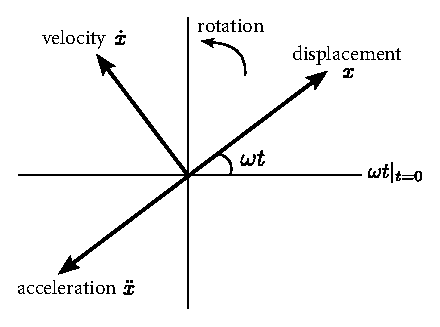
\includegraphics[width=.55\textwidth]{x-v-a.eps}
\end{figure}
\textit{i.e.}, there exists a $\pi/2$ and $\pi$ phase difference between the velocity and displacement, and acceleration and displacement, respectively.\\

Expression the trial solution in Euler's form: $\displaystyle x = x_{0}\cos(\omega t-\phi)=x_{0}e^{j(\omega t -\phi)}$ and substitute into the governing equation:

\begin{equation}
    \underbrace{-\omega^{2}x_{0}e^{j\omega t }e^{-j\phi}}_{\ddot{x}}
    + 2\gamma \omega_{n} \underbrace{j\omega x_{0}e^{j\omega t }e^{-j\phi}}_{\dot{x}}
    +\omega_{n}^{2} \underbrace{x_{0}e^{j\omega t }e^{-j\phi}}_{x}
    =\frac{F_{0}}{m}e^{j\omega t}
\end{equation}

Re-arrange,
\begin{equation} \label{eqn:25}
     \cancel{e^{j\omega t}} e^{-j\phi} (-\omega^{2} x_0 + j2\gamma\omega_{n}\omega x_0 + \omega_{n}^{2} x_0) = \frac{F_{0}}{m} \cancel{e^{j\omega t}}
\end{equation}

What does \autoref{eqn:25} tell us? Well, the term $e^{-\phi j}$ implies an anticlockwise rotation of an angle $\phi$. Therefore, \autoref{eqn:25} can be graphically represented as
\begin{figure}[H]
    \centering
    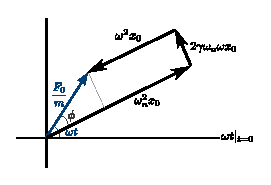
\includegraphics[width=.55\textwidth]{rotation_geo.eps}
\end{figure}
The length of $F_0/m$ (blue) can be parsed into 3 individual trajectories - $\omega_{n}^2 x_0$ is the trajectory of the displacement, $2\gamma\omega_{n}\omega x_0$ is the trajectory of the velocity, and $\omega^2 x_0$ is the trajectory of the acceleration\footnote{Note their directions, and correlates to the figure above!}. \\

Therefore, we can represent the length (\textit{magnitude}) of $x_0$ using Pythagoras' theorem,
\begin{equation}
    \lvert x_{0} \rvert = \frac{F_{0}/m}{\sqrt{(\omega_{n}^{2} \omega^{2})^{2}+(2\gamma\omega_{n}\omega)^{2}}}
\end{equation}
and similarly, the \textit{phase} of $x_0$:
\begin{equation}
    \tan \phi = \frac{2\gamma \omega_{n}\omega}{\omega_{n}^{2}-\omega^{2}} \quad \to \quad \phi = \tan^{-1} \bigg(\frac{2\gamma \omega_{n}\omega}{\omega_{n}^{2}-\omega^{2}}\bigg)
\end{equation}

\hrule \vspace{.5cm}

Let us think about how the relations between $\omega$, $\omega_{n}$, $2\gamma\omega_{n}\omega$ could affect the magnitude response:
\begin{enumerate}
	\item When $\omega\to 0$, 
    \[
        x_{0} = \frac{F_{0}}{m\omega_{n}^{2}}=\frac{F_{0}}{k}
    \] 
    which implies that $x_{0}$ is stiffness controlled.
 
	\item If $\omega\to\infty$, 
    \[
        \omega^{2}=\frac{F_{0}}{mx_{0}} \quad \to \quad x_{0}=\frac{F_{0}}{\omega^{2}m}
    \] 
    which implies that $x_{0}$ is mass controlled.
 
	\item If $\omega_{n}=\omega$, the gradient of the magnitude response $\lvert x_0 \rvert$ with respect to $\omega$ is zero, the peak magnitude of $x_0$ occurs - also known as the \textbf{resonance}. The \textbf{resonance frequency} is represented as: 
    \[
        \omega_{p}=\sqrt{1-2\gamma^{2}}
    \]
\end{enumerate}

% Therefore, the general solution is 
% \[
%     \boxed{x = x_{0}\cos(\omega t +\phi)+A_{1}e^{\mu_{1}t}+A_{2}e^{\mu_{2}t}}
% \]
\end{tcolorbox}

\hrule \vspace{.1cm}
\paragraph{Electrical analogy} The forced oscillation can be generated with the following $L$-$C$-$R$ circuit with an additional periodic voltage source term:
\begin{figure}[H]
    \centering
    \begin{tikzpicture}
    \draw
    (0,0) to[sinusoidal voltage source=\(V_0 \cos \omega t\)] ++(0,2)
                to[R=\(R\)] ++(2,0) 
                to[L=\(L\)] ++(2,0) 
                to[C=\(C\)] ++(0,-2) 
      -- (0,0);
    \end{tikzpicture}
\end{figure}
The governing question of the system shown above is
\[
    L \frac{d^2I}{dt^2} + R\frac{dI}{dt} + \frac{1}{C}I = V_0 \cos \omega t
\]

\end{document}